% !TEX root = ../thesis.tex
% testing and optimization experiments
% @author Tobias Wulf
%

\section{Verhalten bei kombinierten Fehllagen}\label{sec:exp6}

\textbf{Zweck:} Das Experiment soll als Stichprobe dienen und zeigen, dass das Regressionsmodell auch bei kombinierten Fehllagen funktionieren kann. Dafür werden eine Kombination der Parametergrenzen aus dem vorangegangenen Experiment aus \autoref{sec:exp5} übernommen, siehe \autoref{fig:drift-horizontal-model-parms} und \autoref{fig:drift-vertical-model-parms}. So setzt sich für das Rauschniveau $\sigma_n^2$ die Parametergrenzen aus der unteren Grenze für vertikalen Drift und oberen Grenze für horizontalen Drift zusammen. Für die Skalierungsparameter der Kovarianzfunktion, sind die Parametergrenzen aus horizontalem Drift für die Höhenskalierung $\sigma_f^2$ eingestellt. Die Längenskalierung $\sigma_l$ übernimmt ebenfalls die resultierenden Grenzen aus horizontalem Drift. Es sind wieder $N_{Ref} = 17$  Referenzwinkeln für das Regressionsmodell mit euklidischer Abstandsfunktion nach \autoref{eq:de2innorm} und resultierender Kovarianzfunktion nach \autoref{eq:kfun} vorgegeben. Das Modell wird als mittwertfreier Kernel betrieben. Die Durchlaufzahl für die äußere Optimierung nach \autoref{alg:bayesopt} ist mit $10$ Durchläufen wieder verringert. Modelltrainingsdaten basieren auf Vektoren bzw. Skalare.

\textbf{Durchführung:} Das Experiment wird in zwei Durchgängen ausgeführt. Vor jedem Durchgang werden Trainings- und Testdatensatz separat prozessiert und anschließend im Demonstrationsskript geladen. Es wird der Testdatensatz über einfache Mittlung der Daten ausgewertet. Die einfache Mittlung ist vom etwaigen Offset in den Simulationsdaten bereinigt. Es folgt die volle Regressionsmodell-Initialisierung und -Optimierung mittels Trainings- und Testdaten. Danach werden basierend auf den Testdaten die Vorhersage- und Verlust- sowie Fehlerberechnungen ausgeführt. Abschließend sind die Ergebnisse aus Regression und einfacher Mittlung grafisch ausgewertet. Die Testdaten beinhalten in jedem Durchgang $720$ Simulationswinkel bei einer Auflösung von $\SI{0,5}{\degree}$ und bilden eine volle Rotation des Magneten ab. Der Magnet ist in beiden Durchgängen um $\SI{11}{\degree}$ in der $Y$-Achse verkippt. Der $Z$-Abstand beträgt in beiden Durchgängen $4,5$ mm. Im ersten Durchgang ist der Sensor in $X$ um $0,5$ mm und in $Y$ um $1$ mm so verschoben, sodass sich der Magnet noch oberhalb des Sensors befindet. Beim zweiten Durchgang wird der Versatz in $X$ mit $2,5$ mm und für $Y$ mit $2$ mm nochmals erhöht. Der Magnet mit $2$ mm Radius liegt damit räumlich neben dem Sensor.

\textbf{Erzeugte Datensätze:} Jeweils zwei Trainings- und Testdatensätze mit korrespondierenden Positionen des Sensors und Verkippungswinkel des Magneten.

\textbf{Matlab-Skript:} demoGPRModule.m, siehe \autoref{mcode:demogprmodule}.


\clearpage


\textbf{Abweichende Parameter von \autoref{tab:sim-params-exp}:}

\begin{itemize}
	\item TrainingsOptions: nAngles: 17
	\item TrainingsOptions/ TestOptions: (xPos; yPos; zPos): 
	\begin{itemize}
		\item[a.] $(0,5;1;4,5)$
		\item[b.] $(2,5;2;4,5)$
	\end{itemize}
	\item TrainingsOptions/ TestOptions: tilt: $11$
	\item GRPOptions: kernel : 'QFCAPX'
	\item GRPOptions: $\sigma_f^2$-Bounds: $(0.4,20)$
	\item GRPOptions: $\sigma_l$-Bounds: $(4,40)$
	\item GRPOptions: $\sigma_n^2$-Bounds: $(3\cdot10^{-7},10^{-5})$
	\item GPROptions: mean: 'zero'
	\item GRPOptions: OptimRuns: 10
\end{itemize}

\textbf{Ergebnisse:} Die Ergebnisse beider Durchgänge sind in \autoref{fig:kombinierte-fehllagen-gpr} und \autoref{fig:kombinierte-fehllagen-sensor} grafisch gegenübergestellt. \autoref{fig:kombinierte-fehllagen-gpr} zeigt die Reaktion des Regressionsmodells und resultierende absolute Winkelfehler auf die kombinierten Fehllagen aus räumlichen Versatz und Verkippung des Magneten. Als ergänzende Darstellung zeigt \autoref{fig:kombinierte-fehllagen-sensor} die Reaktion des Sensor-Arrays in Bezug auf die gezeigten Beispiele in \autoref{fig:kombinierte-fehllagen-gpr}.


\clearpage


\textbf{Beobachtungen:} Für die Fehllage a) in \autoref{fig:kombinierte-fehllagen-gpr} zeigt sich, dass das Regressionsmodell diese sehr gut kompensieren konnte. Die Kovarianzmatrix zeigt ein homogenes Funktionsabbild für jeden Trainingspunkt zueinander mit nur sehr kleinen Abweichungen. Der Matrixmittelwert liegt mittig zu den einzelnen Kurvenverläufen. Die Kurvenverläufe besitzen eine gleichmäßige nicht spitz zulaufende Glockenform. Das Verhältnis aus Höhen- und Längenskalierung der Kovarianzfunktion liegt ca. bei $1:10$. Das Rauschniveau ist in der Optimierung gegen seine unter Parametergrenze gelaufen. Jedes Training-Sample hat dadurch annähernd den gleichen Einfluss in der Regression. Das Modell besitzt in Bezug auf die Trainingsdaten und unter Berücksichtigung des Parameterverhältnisses eine mittlere Komplexität \cite{Rasmussen2006}. Es stellt sich eine hohe Generalisierung mit $MSLLA$ und $MSLLR$ kleiner $-5$ ein. Es gibt leichte Schwankungen in der Generalisierung und zwei markante Ausreißer, die aber alle negativ sind und somit wenig bis mäßig vom Generalisierungniveau abweichen. Die Vorhersage ist sehr vertrauensvoll über die gesamte Rotation hinweg mit annähernd konstanten sehr engen Konfidenzintervallen für die Winkelvorhersage und Radius. Leichte Schwankungen in den Konfidenzintervallen entsprechen den Schwankungen der Modellverluste. Der mittlere Winkelfehler geht mit $\SI{0,4}{\degree}$ gegen null. Der maximale Winkelfehler ist mit $\SI{0,17}{\degree}$ sehr klein und taucht an der Peak-Stelle des Generalisierungsausreißers bei ca. $\SI{220}{\degree}$ auf. In der ergänzenden Ergebnisansicht in \autoref{fig:kombinierte-fehllagen-sensor} a) zeigt die polare Darstellung der Simulationsergebnisse, dass die einfache Mittlung der Daten zwar eine Kreisbahn ergibt, diese aber nicht zentriert ist. Das Regressionsmodell gleicht diese Fehllage vollständig aus. Die Streuung der Sensor-Pixel auf dem Kennfeld deckt annähernd den vollen nichtlineare Bereich des Kennfeldes ab. Die Sensor-Pixel überlagern sich teilweise. Das Sensor-Pixel mit der Koordinate $(1,8)$ liegt dabei an der Grenze zum linearen Bereich des Kennfeldes. Die Auswertung der einzelnen Sensor-Pixel-Kreisbahnen zeigen, dass sich erste Darstellungsprobleme an der Sensor-Pixel-Koordinate $(1,8)$ und angrenzende Pixel einstellen. Hervorgerufen durch die stärkere Verzerrung der Feldstärkenverläufe von Kreisbahnen zu Ellipsoiden.
\newline
Mit der Fehllage b) in \autoref{fig:kombinierte-fehllagen-gpr} hat das Regressionsmodell Schwierigkeiten diese zu kompensieren. Das Skalierungsverhältnis von Höhen- zu Längenparameter liegt ca. bei $7:50$. Die Kurvenverläufe sind stark inhomogen und  sind wechselhaft zwischen breiten Glocken- und Keilformen. Der Matrixmittelwert ist abgesenkt. In Bezug auf die Trainingsdaten und Parameterverhältnis stellt sich damit z.T. eine hohe Modellkomplexität ein, die für einige Trainingsdaten durch keilförmige Kurven durchbrochen ist  \cite{Rasmussen2006}. Mit einfachen Worten, das Regressionsmodell kann sich nicht auf die stark variierenden Daten einstellen, sodass der versuchte Kompromiss in der Komplexität fehlschlägt. Das Generalisierungsniveau ist negativ und von der Mittlung bei ca. $-4$ zufriedenstellend, allerdings abschnittsweise in Gänze aufgehoben, sodass nur der Fit auf den Trainingsdaten erhalten bleibt. Die Ursache dafür ist die Keilform an den jeweiligen Trainingsdatenpunkten in der Kovarianzmatrix. Der Bruch in der Generalisierung ist zwischen $\SI{0}{\degree}$ und $\SI{110}{\degree}$ sowie zwischen $\SI{150}{\degree}$ und $\SI{275}{\degree}$ zu beobachten. Gleichmaßen zeigen sich Einbußen für die Generalisierung in der Vertrauensaussage über die Konfidenzintervalle wieder. Dies ist durch ein Aufschwingen der Intervalle in den angegebenen Abschnitten zu sehen. Der Winkelfehler folgt entsprechend der Generalisierung und dem Konfidenzintervall. Der mittlere Fehler hat sich erhöht auf $\SI{0,33}{\degree}$, der maximale liegt nun bei rund $\SI{2}{\degree}$. Die Ergänzung in \autoref{fig:kombinierte-fehllagen-sensor} b) zeigt die Verzerrung der Testdaten in einfacher Mittlung zu einer nicht kreisförmigen oder ellipsenähnlichen Bahn führen. Das Regressionsmodell schafft es nicht die stark verzerrte Kreisbahn zu kompensieren. Die Sensor-Pixel-Ansicht auf dem Cosinus-Kennfeld zeigt, dass die Pixel-Überlagerung vollständig aufgehoben ist und die Streuung der Pixel vom nichtlinearen Kennfeldbereich über den lineare bis hin zur Kennfeldmitte nahe $\SI{0}{\kilo\ampere\per\metre}$ reicht. Die jeweiligen Feldstärkenverläufe sind alle zu Ellipsen gestaucht und werden im Bereich der Sensor-Pixel-Koordinate $(1,8)$ so stark gestaucht, dass sie nun mehr als Linien wahrnehmbar sind. Das resultiert für die Betrachtung der Ausgangsspannungen zu stark verzerrten und größtenteils nicht kreis- oder ellipsenförmigen Bahnverläufen.


\clearpage
\begin{figure}[tbph]
	\centering
	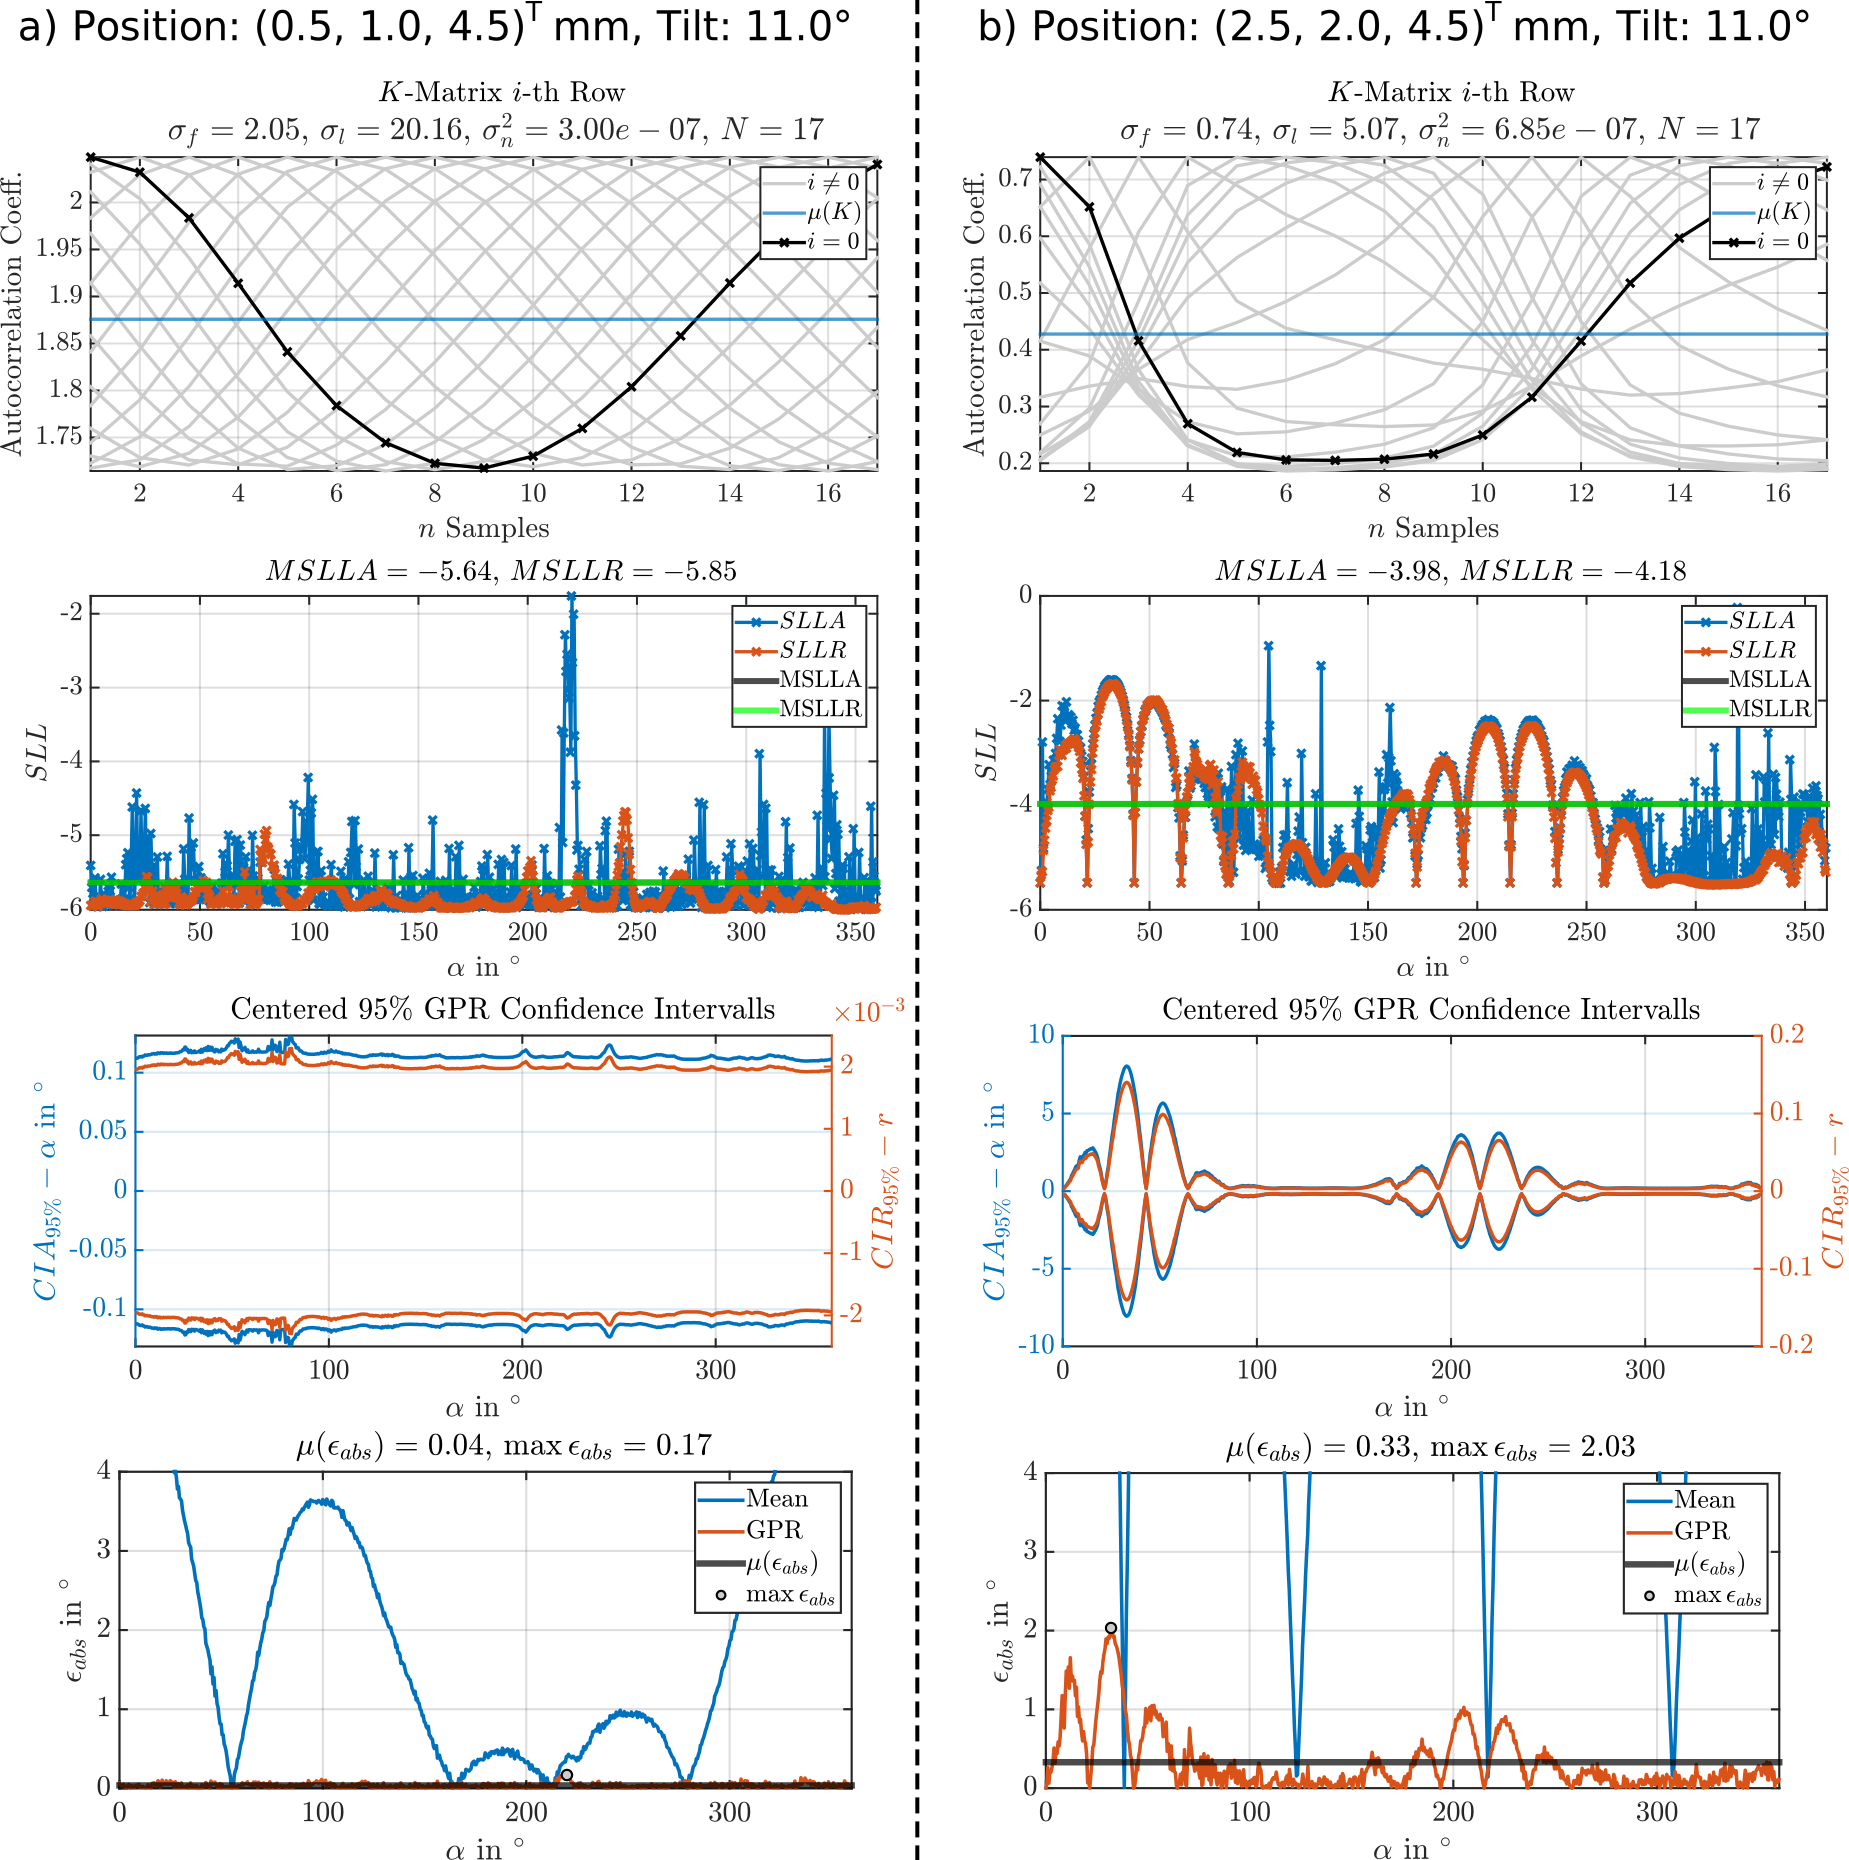
\includegraphics[width=\linewidth]{chapters/images/4-EuOExp/Kombinierte-Fehllagen-GPR}
	\caption[Beispiel kombinierter Fehllagen in der Regressionsansicht]{Beispiel kombinierter Fehllagen in der Regressionsansicht. Gezeigt sind zwei Fehllagen mit gleicher Magnetverkippung und $Z$-Abstand zum Magneten. Für a) befindet sich der Magnet räumlich über den Sensor. Für b) liegt der Sensor räumlich neben dem Magneten. Der Magnetradius beträgt $2$ mm. Beide Beispiele sind mit voll optimierten Modell nach \autoref{alg:fminconopt} und \autoref{alg:bayesopt} und gleicher Konfiguration ausgeführt worden. Genutzt ist der Kernel nach \autoref{eq:kfun} mit Abstandsfunktion nach \autoref{eq:de2innorm}. Die Referenzwinkelanzahl beträgt $N_{Ref} = 17$. Gezeigt sind: Die Kovarianzmatrix aufgetragen für jede $i-te$ Matrixreihe inklusive Matrixmittelwert. Die Generalisierung über den standardisierten logarithmischen Verlust (engl. Loss) $SLL$, jeweils für Winkel $SLLA$ und Radius $SLLR$, sowie die resultierende Verlustmittlung $MSLLA$ und $MSLLR$. Die $95\%$ Konfidenzintervalle aus Winkelvorhersage $CIA_{95\%}$ und Radius $CIR_{95\%}$. Der absolute Winkelfehler durch Mittlung (Mean) und Gauß-Prozess-Regression (GPR).}
	\label{fig:kombinierte-fehllagen-gpr}
\end{figure}


\clearpage
\begin{landscape}
\begin{figure}[tbph]
	\centering
	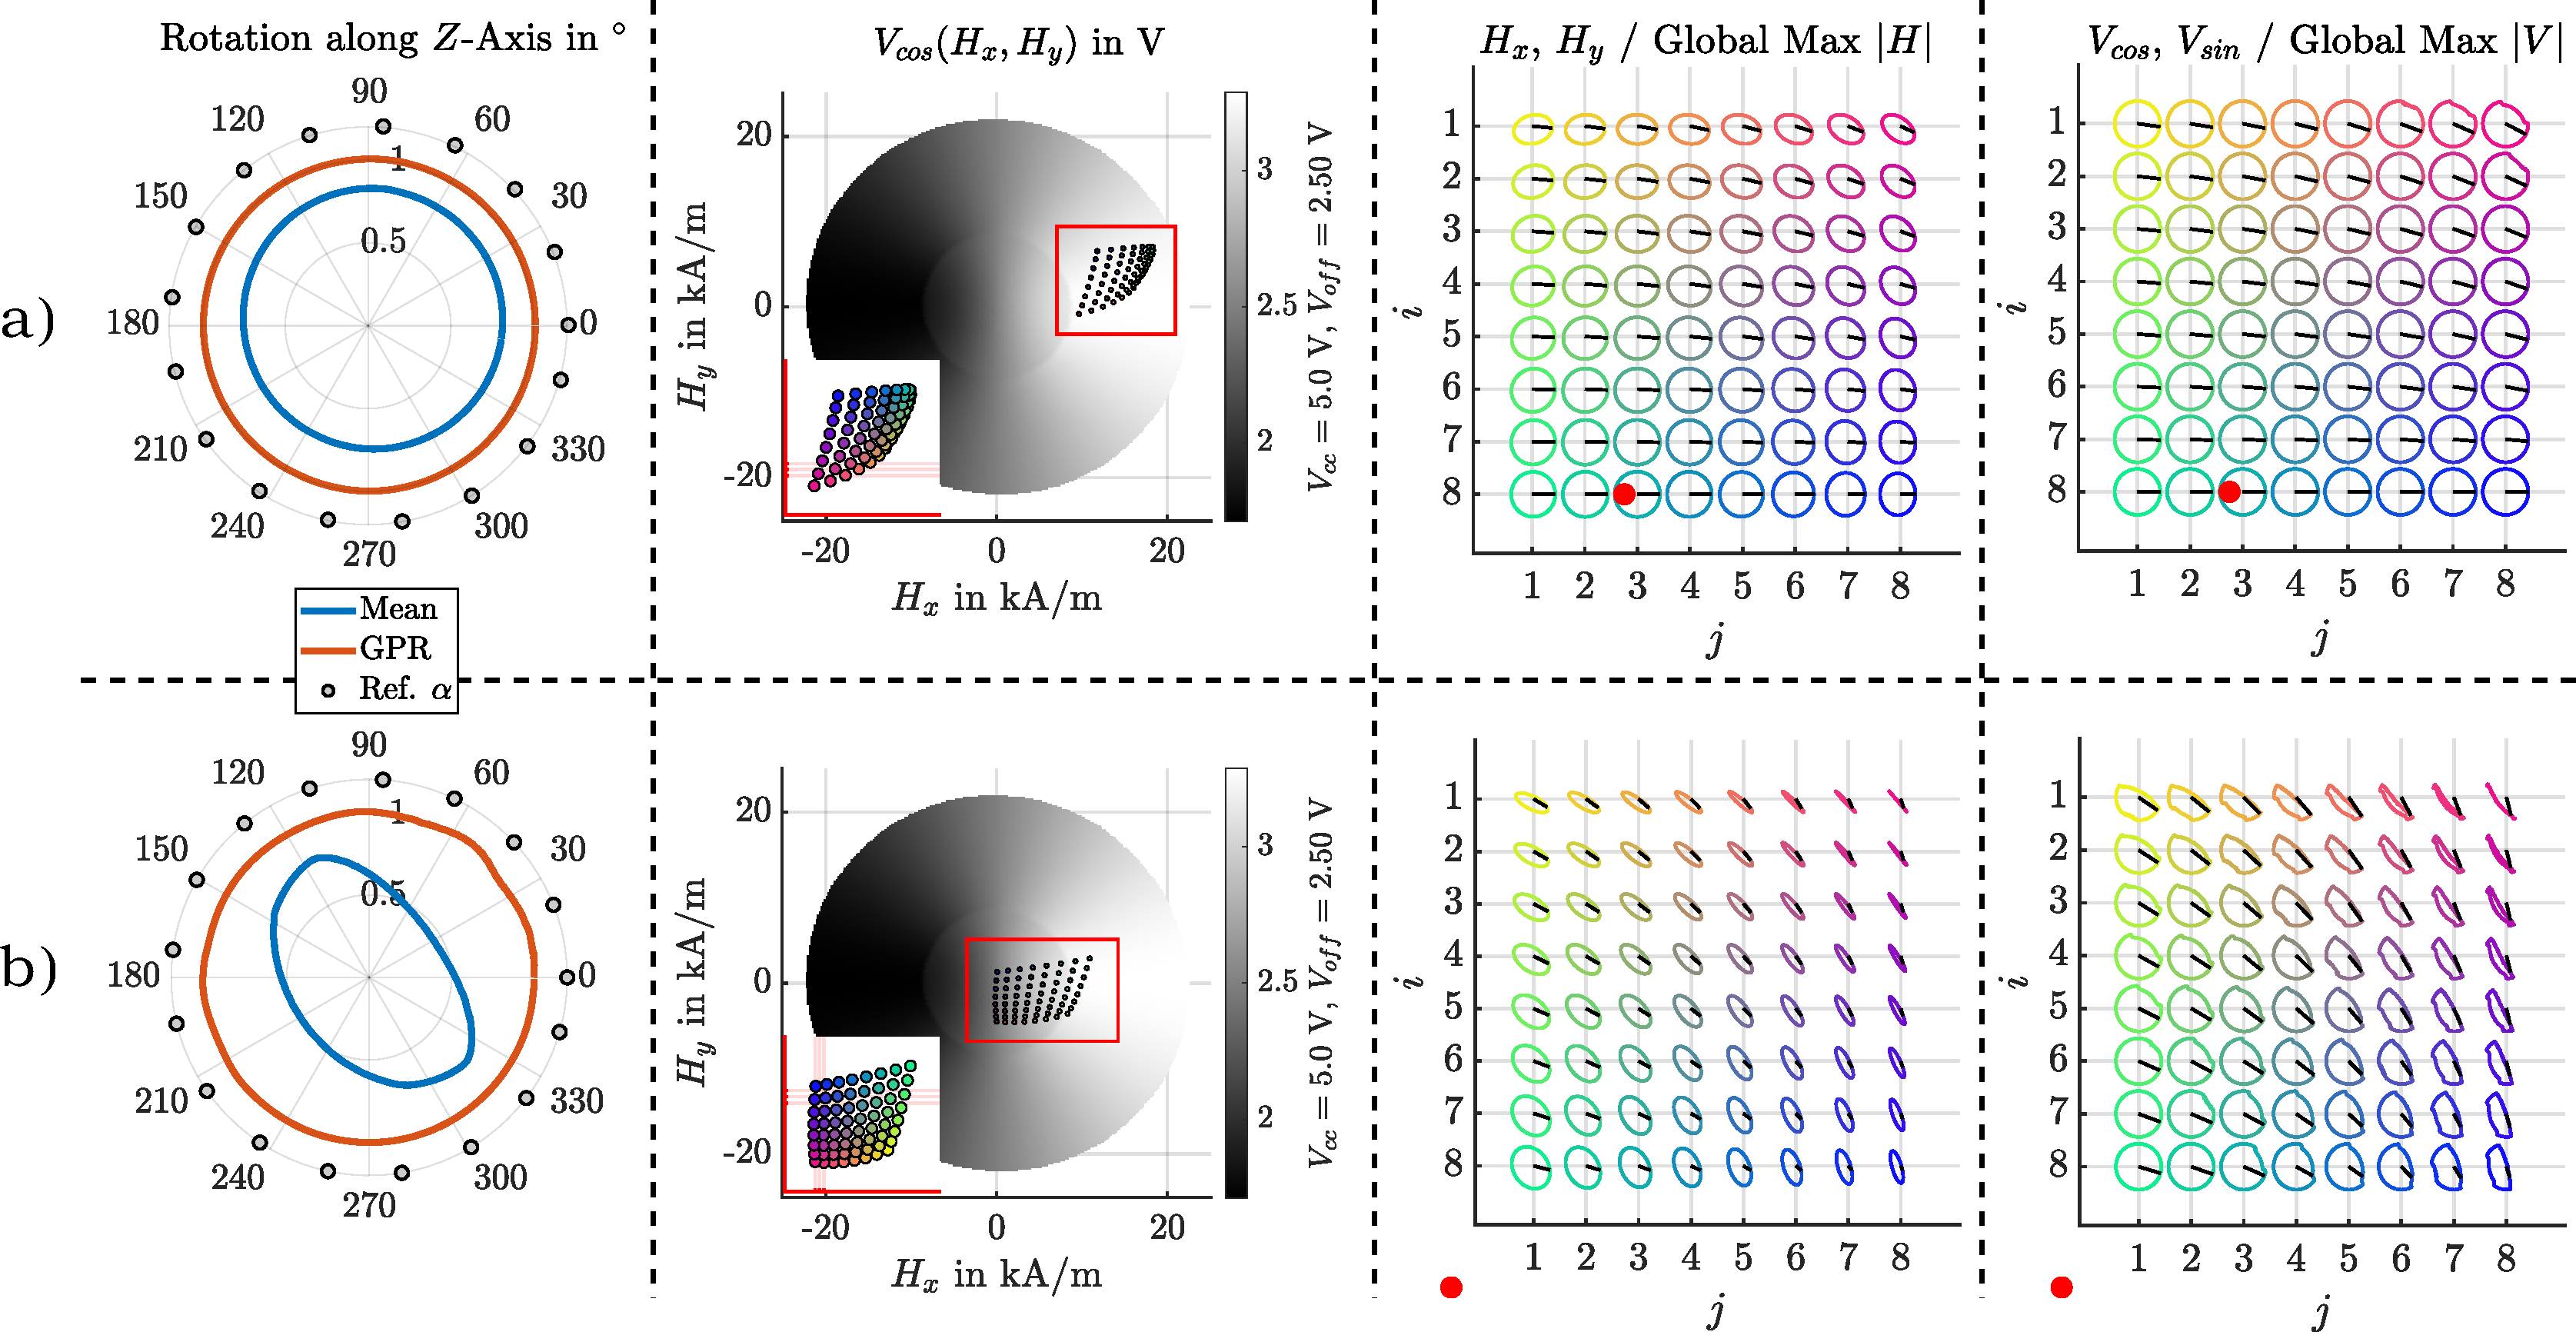
\includegraphics[width=.85\linewidth]{chapters/images/4-EuOExp/Kombinierte-Fehllagen-Sensor}
	\caption[Beispiel kombinierter Fehllagen aus Sicht des Sensor-Arrays]{Beispiel kombinierter Fehllagen aus Sicht des Sensor-Arrays. Ergänzung zur \autoref{fig:kombinierte-fehllagen-gpr}. Die Fälle a) und b) korrespondieren zu den gezeigten Beispielen in \autoref{fig:kombinierte-fehllagen-gpr}. Gezeigt sind: Die polare Darstellung aus einfacher Mittlung (Mean) der Testdaten und Ergebnis der Gauß-Prozess-Regression (GPR) inkl. Anzeige der Referenzwinkel. Das Streuungsmuster der Sensor-Pixel auf dem Kennfeld der Cosinus-Funktion für den Simulationswinkel $\alpha = \SI{21,5}{\degree}$. Die $H_x$- und $H_y$-Feldstärkenverläufe normiert auf die globale maximale Betragsfeldstärke $|H|$ aller simulierten Feldstärken. Die Simulationsergebnisse der Sensor-Array-Simulation für Cosinus- und Sinus-Ausgangsspannungen normiert auf das globale Betragsmaximum $|V|$, als resultierendes Betragsmaximum aller simulierten Ausgangsspannungen. Beide Ansichten zur Feldstärke und Spannung bilden die gleichen Sensor-Pixel-Positionen  bei voller Magnetrotation ab. Die Farbgebung entspricht der Pixel-Darstellung auf dem Kennfeld. Die Magnetposition ist in a) und b) rot hervorgehoben. In b) befindet das Sensor-Array neben dem Magneten, die Position ist daher nur angedeutet.}
	\label{fig:kombinierte-fehllagen-sensor}
\end{figure}	
\end{landscape}


\clearpage

